\documentclass[a4paper,3p,sort&compress]{elsarticle}

\usepackage[draft]{hyperref}
\usepackage{url}
\usepackage{booktabs}
\usepackage{graphicx}
\usepackage{xspace} 
\usepackage{booktabs}
\usepackage{makecell}
\usepackage{lineno}
\usepackage{natbib}
\usepackage{amsmath}
\DeclareRobustCommand{\citeext}[1]{\citeauthor{#1}~\cite{#1}}

\usepackage[nomargin,inline,draft]{fixme}
\fxsetup{theme=color,mode=multiuser}
\FXRegisterAuthor{j}{jla}{\color{purple}JLA}
\FXRegisterAuthor{s}{spv}{\color{teal}SPV}

\journal{-}

%% `Elsevier LaTeX' style
\bibliographystyle{plain}
%%%%%%%%%%%%%%%%%%%%%%%

\begin{document}
\linenumbers

% Macro para escribir NO$_2$
\newcommand{\no}{NO\textsubscript{2}\xspace}

\begin{frontmatter}

  \title{Pollution Forecast: Introducing a novel visualization technique for time series uncertainty visualization}


  \author{Sebasti\'an P\'erez Vasseur}
  \author{Jos\'e L. Aznarte}
  \address{Artificial Intelligence Department\\Universidad Nacional de
    Educaci\'on a Distancia --- UNED\\c/ Juan del Rosal, 16, Madrid, Spain}
  \ead{jlaznarte@dia.uned.es}
  

\begin{abstract}
  
\end{abstract}

\begin{keyword}
probabilistic forecasting \sep visualization \sep dotplot
\end{keyword}

\end{frontmatter}

%\linenumbers

\section{Introduction}
\label{sec:intro}

\jnote{Usa bibtex+referencias para las citas.} Hothorn \emph{et al.} stated that
the real objective in a machine learning regression analysis is to find the full
conditional distribution of the target variable.\jnote{Es una afirmación
  demasiado general como para asignarla a un único autor. Diría que es algo más
  generalizado.} Currently, many machine learning models only provide a point
distribution, which is usually the expected value of the target variable. Then
the users of the model must take a decision based on this single predicted
estimation. However, only point information without uncertainty creates a false
sense of deterministic result that can lead to false confidence in the decision.
That's why as noted by Fernandez et Al., uncertainty improves decision making.
However, as we will see, the typical visualization tools that users rely on are
not really suited for probabilistic information, as they are designed for
deterministic information. This also adds an additional difficulty for this
charts \jnote{No se entiende a qué ``this charts'' te refieres}. Users do not
read a single value but have to determine the probability of the target value
within a certain range.

If we focus on categorical data, the standard visualization tool is the bar or
column chart. As is known, this particular chart uses a rectangle as marker and
encodes the category as the x-axis and the target value as the y-axis (or vice
versa). If we wish to add probabilistic information to the chart, we could add
error bars to the already present bars. However as noted by Kai et Al. the
information should be intrinsic to the visualization. Therefore we should think
of a different way to display the uncertainty in the target.

Several approaches exist already. The most straightforward solution is the
violin plot \jnote{Antes que el violín, ¿no sería mejor hablar del diagrama de
  cajas, que es más sencillo y más antiguo? Añadiría a la lista el histograma y
  la estimación KDE.} which displays the probability density function for each
category. As Fernandez et Al. states, users do not tend to have enough
statistical knowledge to interpret this type of chart making it difficult to
extract information. The other solution is the box plot, introduced by Tukey et
al. in 1977. This type of chart uses a rectangle which top and bottom parts show
the 1st and 3rd quantile of the target value for each category and a line to
show the 2nd quantile. This chart is much simpler to read and has been showcased
as the main solution to show uncertainty or probability distribution. The boxen
plot brings additional rectangles per category that enable to show more
percentiles than the box plot.

\section{Time Series probabilistic charts}
\label{sec:time_series}

Time series data representation could be a subset of categorical data visualization where the categories are the ordered time slots. 
Therefore, we could apply the solutions seen above to represent probabilistic time series data. Usually the number of time categories
is high and we have to deal with limited space per category. Therefore, this constraint rules out the violin plot. However, the use of boxen plots for time series has been showcased specially for EPS diagrams, very used for meteorological data.

However, time series data have usually been represented with a dedicated type of chart: line charts, where the marker is a 
line where the x-axis represent time and the y-axis represents the target value. Also, we could use error bars to represent uncertainty,
but other intrinsic solutions are being used. The first one is to represent the confidence interval, where instead of a single line, we 
will draw 3 lines: the first one for the 5\% percentile, the second one for the mean and the third one for the 95\% percentile. 
Another solution is the gradient chart where colour areas represent each of the
deciles of the probabilistic time series.

However Kay et Al. \cite{kay_when_2016} investigation noted that users prefer to think in terms of natural frecuencies (2/10) instead 
of probabilities (.2), and therefore it's better to use discrete outcomes to communicate probabilities. All the charts above 
represent probabilities or percentile and a discrete solution would improve readability and understanding of the charts: We
propose therefore a novel visualization technique to show time series data: time series dot plot. 

This chart would draw a dot for each of the deciles of the target variable. This simplifies the readability of the chart as
users just need to count the number of dots to estimate approximately the natural frequencies.

Figure \ref{figure:charts} shows a summary of the main types of probabilistic time series charts.

\begin{figure}
  \centering
  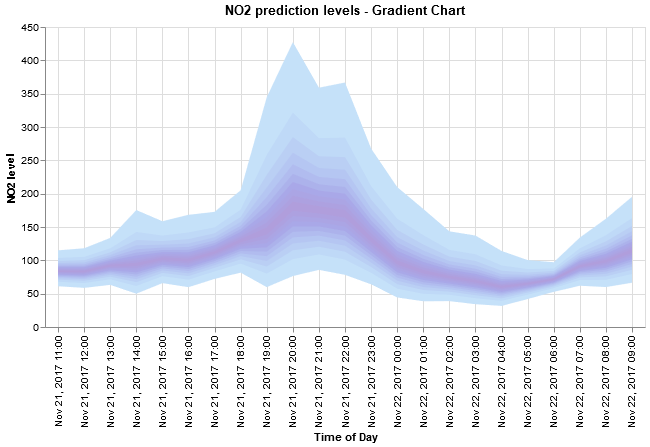
\includegraphics[width=0.4\textwidth]{gradient} 
  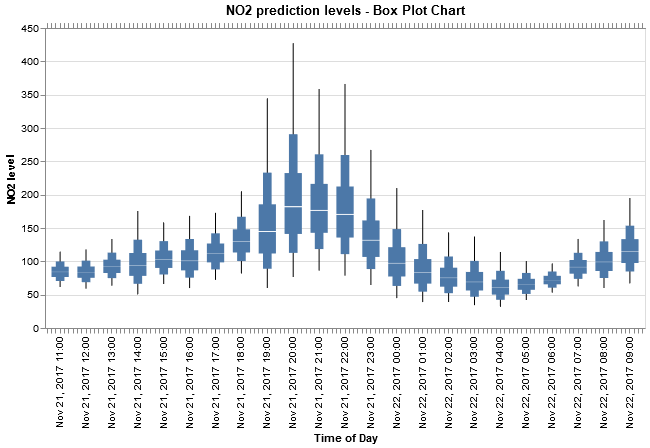
\includegraphics[width=0.4\textwidth]{boxplot}
  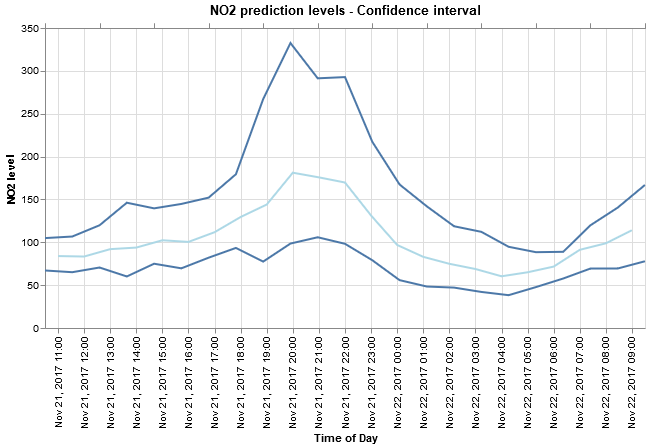
\includegraphics[width=0.4\textwidth]{ci} 
  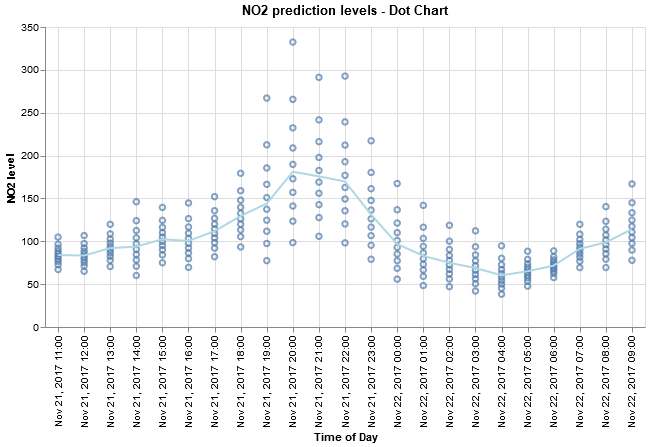
\includegraphics[width=0.4\textwidth]{dot}
  \caption{\label{figure:charts} Probabilistic Time Series Chart. 
  Top Left: Gradient Chart. Top Right: Box Plot. 
  Bottom Left: Confidence Interval. Bottom Right: Dot Chart.  }
\end{figure}

\subsection{Application: No levels forecast in Madrid}

Air quality has become a concern in recent years and lately pollution peaks have forced local authorities to take measures like cutting traffic or blocking certain city areas. Those measures are purely reactive and therefore a forecast of pollution might be preferrable as proactive measures could be taken and prevent the pollution peak before it happens.

Several stations in Madrid record the levels of NO in different parts of the city. We use a probabilistic
machine learning model to predict the levels of No in one of the stations. Instead of providing a point estimate, it provides a 
probability distribution at each of the prediction horizons. We represent the predictions. in a chart. This chart will be used by the
authorities whenever a decision must be reached regarding the levels of pollution and preventive actions to be taken.

\section{Experimental Design}
\label{sec:exp_design}

We would like to compare the readability of the four main types of probabilistic time series charts displayed in figure 
\ref{figure:charts}. We will evaluate how well the charts can help answering a probability question regarding the NO levels.

For this, we will request the participation of users through the Amazon Mechanical Turk website. Those users will perform a small task
in exchange for a small fee (few dollars): the assigned task is a test where we measure how well can the participants read the charts.
As suggested by Brenner et al., we will be selecting Masters Level Participants. We will be testing 20 users per type of chart 
and as each is answering 5 questions, we will have 100 answers per type of chart.

For each type of chart, we designed a test with a presentation part where we explain how the charts can be read and a questions part
with 5 probability questions. As an example, we show in figure \ref{figure:explanation} the presentation part of the time series 
dot chart. The questions
require reading the chart to estimate the probability of the NO levels inside a certain range. We will then measure for each question
the error in the estimation and the time it took to answer. Inspired by the work of Brenner et al., we are also asking at the end of 
the survey how difficult was reading the chart and how confident are they with their answers. 

\begin{figure}
  \centering
  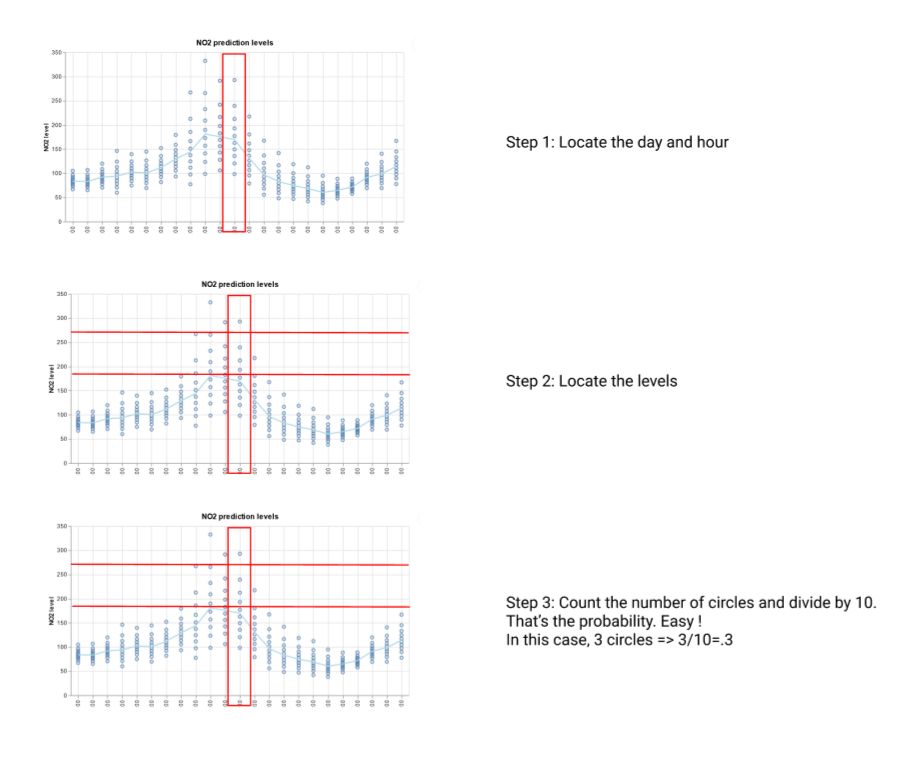
\includegraphics[width=0.4\textwidth]{dot_explanation}
  \caption{\label{figure:explanation} Image explaining how the chart is read.  }
\end{figure}

\section{Results}
\label{sec:results}

Figure \ref{figure:errors} shows the histogram of the absolute value of the probability errors in percentage. 
Although the majority 
of users report errors on the 0-20\% section, the dot chart almost has no errors outside of this band. 
Also, we did not see an improvement in 
the error rate as users were answering questions, therefore we combined all errors together.

\begin{figure}
  \centering
  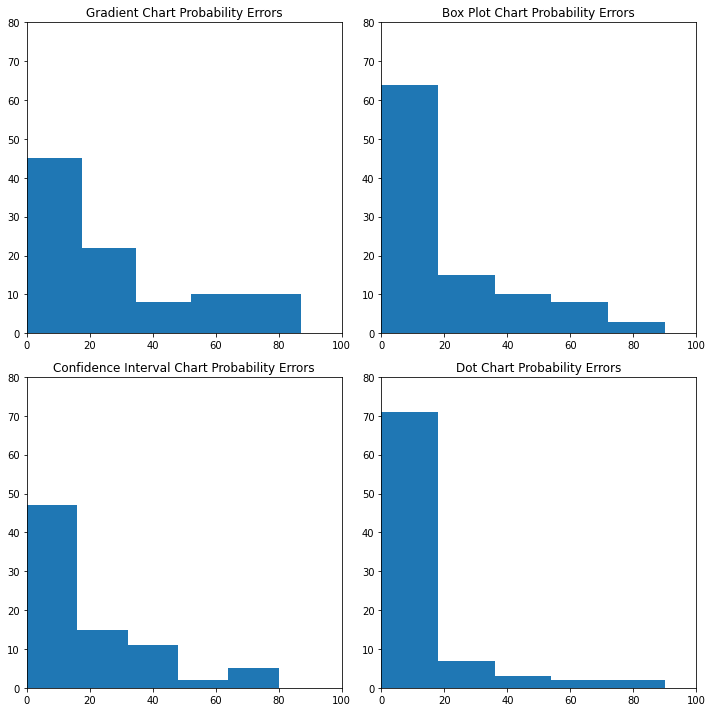
\includegraphics[width=0.6\textwidth]{probability_errors}
  \caption{\label{figure:errors}Distribution of absolute error for all questions per type of chart.}
\end{figure}

However, users seem to reflect their learning in the time it takes to read 
and answer the question. we see in figure \ref{figure:duration} that for every chart, the time it takes 
to read and answer the question decreases for every question answered. We also did not see 
noticeable difference between the type of charts. However, the difficulty of reading the chart might impact 
this number for a higher number of questions.

\begin{figure}
  \centering
   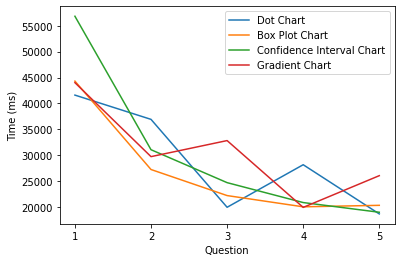
\includegraphics[width=0.6\textwidth]{duration_evo}
  \caption{\label{figure:duration} Median Time it took to answer each question for each of the types of chart.}
\end{figure}  

Confidence and load also prove the superior performance of the time series dot chart. 
Figure \ref{figure:confi_load} shows how the dot chart reports higher levels of confidence and 
lower levels of load of difficulty.

\begin{figure}
  \centering
   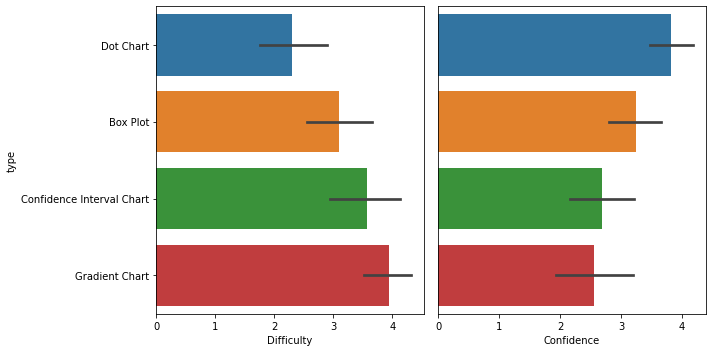
\includegraphics[width=0.5\textwidth]{confi_load}
  \caption{\label{figure:confi_load} Difficu mjkiulty (left) and Confidence (right) in reading and answering the questions for each chart}
\end{figure}

We also see a lack of statistical knowledge from standard users as some users were reporting 
probabilities above 1, showing they do not understand the basic theory of statistics. 
We reported 9 users from 80 whose answers could not be used as their answers could not be 
applicable (probability higher than 1 or text).

\section{Conclusions}
\label{sec:concl}

We have compared 4 probabilistic time 
series charts when answering a quantitative probability question: 
gradient time series chart, box plot time series chart, confidence interval 
time series chart and time series dot chart.
We have applied them to the field of \no pollution levels probabilistic 
time series as an application example and to build the user tests.
We enrolled a panel of volunteers and asked them to read the charts 
and determine the probability of \no to be in a certain interval at a certain 
hour.
All users learned to use the charts and after 5 questions all charts 
need almost the same amount 
of time to be read.
However, the results show that users have the highest accuracy when using 
the time series dot chart. Also this chart represents the easiest method 
to get the answer while also providing the highest confidence in the answer.


\section{References}
\label{sec:ref}


\bibliography{refs}

\end{document} 

